
%% bare_conf.tex
%% V1.3
%% 2007/01/11
%% by Michael Shell
%% See:
%% http://www.michaelshell.org/
%% for current contact information.
%%
%% This is a skeleton file demonstrating the use of IEEEtran.cls
%% (requires IEEEtran.cls version 1.7 or later) with an IEEE conference paper.
%%
%% Support sites:
%% http://www.michaelshell.org/tex/ieeetran/
%% http://www.ctan.org/tex-archive/macros/latex/contrib/IEEEtran/
%% and
%% http://www.ieee.org/

%%*************************************************************************
%% Legal Notice:
%% This code is offered as-is without any warranty either expressed or
%% implied; without even the implied warranty of MERCHANTABILITY or
%% FITNESS FOR A PARTICULAR PURPOSE! 
%% User assumes all risk.
%% In no event shall IEEE or any contributor to this code be liable for
%% any damages or losses, including, but not limited to, incidental,
%% consequential, or any other damages, resulting from the use or misuse
%% of any information contained here.
%%
%% All comments are the opinions of their respective authors and are not
%% necessarily endorsed by the IEEE.
%%
%% This work is distributed under the LaTeX Project Public License (LPPL)
%% ( http://www.latex-project.org/ ) version 1.3, and may be freely used,
%% distributed and modified. A copy of the LPPL, version 1.3, is included
%% in the base LaTeX documentation of all distributions of LaTeX released
%% 2003/12/01 or later.
%% Retain all contribution notices and credits.
%% ** Modified files should be clearly indicated as such, including  **
%% ** renaming them and changing author support contact information. **
%%
%% File list of work: IEEEtran.cls, IEEEtran_HOWTO.pdf, bare_adv.tex,
%%                    bare_conf.tex, bare_jrnl.tex, bare_jrnl_compsoc.tex
%%*************************************************************************

% *** Authors should verify (and, if needed, correct) their LaTeX system  ***
% *** with the testflow diagnostic prior to trusting their LaTeX platform ***
% *** with production work. IEEE's font choices can trigger bugs that do  ***
% *** not appear when using other class files.                            ***
% The testflow support page is at:
% http://www.michaelshell.org/tex/testflow/



% Note that the a4paper option is mainly intended so that authors in
% countries using A4 can easily print to A4 and see how their papers will
% look in print - the typesetting of the document will not typically be
% affected with changes in paper size (but the bottom and side margins will).
% Use the testflow package mentioned above to verify correct handling of
% both paper sizes by the user's LaTeX system.
%
% Also note that the "draftcls" or "draftclsnofoot", not "draft", option
% should be used if it is desired that the figures are to be displayed in
% draft mode.
%
\documentclass[conference]{IEEEtran}
% Add the compsoc option for Computer Society conferences.
%
% If IEEEtran.cls has not been installed into the LaTeX system files,
% manually specify the path to it like:
% \documentclass[conference]{../sty/IEEEtran}





% Some very useful LaTeX packages include:
% (uncomment the ones you want to load)


% *** MISC UTILITY PACKAGES ***
%
%\usepackage{ifpdf}
% Heiko Oberdiek's ifpdf.sty is very useful if you need conditional
% compilation based on whether the output is pdf or dvi.
% usage:
% \ifpdf
%   % pdf code
% \else
%   % dvi code
% \fi
% The latest version of ifpdf.sty can be obtained from:
% http://www.ctan.org/tex-archive/macros/latex/contrib/oberdiek/
% Also, note that IEEEtran.cls V1.7 and later provides a builtin
% \ifCLASSINFOpdf conditional that works the same way.
% When switching from latex to pdflatex and vice-versa, the compiler may
% have to be run twice to clear warning/error messages.






% *** CITATION PACKAGES ***
%
%\usepackage{cite}
% cite.sty was written by Donald Arseneau
% V1.6 and later of IEEEtran pre-defines the format of the cite.sty package
% \cite{} output to follow that of IEEE. Loading the cite package will
% result in citation numbers being automatically sorted and properly
% "compressed/ranged". e.g., [1], [9], [2], [7], [5], [6] without using
% cite.sty will become [1], [2], [5]--[7], [9] using cite.sty. cite.sty's
% \cite will automatically add leading space, if needed. Use cite.sty's
% noadjust option (cite.sty V3.8 and later) if you want to turn this off.
% cite.sty is already installed on most LaTeX systems. Be sure and use
% version 4.0 (2003-05-27) and later if using hyperref.sty. cite.sty does
% not currently provide for hyperlinked citations.
% The latest version can be obtained at:
% http://www.ctan.org/tex-archive/macros/latex/contrib/cite/
% The documentation is contained in the cite.sty file itself.






% *** GRAPHICS RELATED PACKAGES ***
%
\ifCLASSINFOpdf
  \usepackage[pdftex]{graphicx}
  % declare the path(s) where your graphic files are
  % \graphicspath{{../pdf/}{../jpeg/}}
  % and their extensions so you won't have to specify these with
  % every instance of \includegraphics
  % \DeclareGraphicsExtensions{.pdf,.jpeg,.png}
\else
  % or other class option (dvipsone, dvipdf, if not using dvips). graphicx
  % will default to the driver specified in the system graphics.cfg if no
  % driver is specified.
   \usepackage[dvips]{graphicx}
  % declare the path(s) where your graphic files are
  % \graphicspath{{../eps/}}
  % and their extensions so you won't have to specify these with
  % every instance of \includegraphics
  % \DeclareGraphicsExtensions{.eps}
\fi
% graphicx was written by David Carlisle and Sebastian Rahtz. It is
% required if you want graphics, photos, etc. graphicx.sty is already
% installed on most LaTeX systems. The latest version and documentation can
% be obtained at: 
% http://www.ctan.org/tex-archive/macros/latex/required/graphics/
% Another good source of documentation is "Using Imported Graphics in
% LaTeX2e" by Keith Reckdahl which can be found as epslatex.ps or
% epslatex.pdf at: http://www.ctan.org/tex-archive/info/
%
% latex, and pdflatex in dvi mode, support graphics in encapsulated
% postscript (.eps) format. pdflatex in pdf mode supports graphics
% in .pdf, .jpeg, .png and .mps (metapost) formats. Users should ensure
% that all non-photo figures use a vector format (.eps, .pdf, .mps) and
% not a bitmapped formats (.jpeg, .png). IEEE frowns on bitmapped formats
% which can result in "jaggedy"/blurry rendering of lines and letters as
% well as large increases in file sizes.
%
% You can find documentation about the pdfTeX application at:
% http://www.tug.org/applications/pdftex





% *** MATH PACKAGES ***
%
%\usepackage[cmex10]{amsmath}
% A popular package from the American Mathematical Society that provides
% many useful and powerful commands for dealing with mathematics. If using
% it, be sure to load this package with the cmex10 option to ensure that
% only type 1 fonts will utilized at all point sizes. Without this option,
% it is possible that some math symbols, particularly those within
% footnotes, will be rendered in bitmap form which will result in a
% document that can not be IEEE Xplore compliant!
%
% Also, note that the amsmath package sets \interdisplaylinepenalty to 10000
% thus preventing page breaks from occurring within multiline equations. Use:
%\interdisplaylinepenalty=2500
% after loading amsmath to restore such page breaks as IEEEtran.cls normally
% does. amsmath.sty is already installed on most LaTeX systems. The latest
% version and documentation can be obtained at:
% http://www.ctan.org/tex-archive/macros/latex/required/amslatex/math/





% *** SPECIALIZED LIST PACKAGES ***
%
%\usepackage{algorithmic}
% algorithmic.sty was written by Peter Williams and Rogerio Brito.
% This package provides an algorithmic environment fo describing algorithms.
% You can use the algorithmic environment in-text or within a figure
% environment to provide for a floating algorithm. Do NOT use the algorithm
% floating environment provided by algorithm.sty (by the same authors) or
% algorithm2e.sty (by Christophe Fiorio) as IEEE does not use dedicated
% algorithm float types and packages that provide these will not provide
% correct IEEE style captions. The latest version and documentation of
% algorithmic.sty can be obtained at:
% http://www.ctan.org/tex-archive/macros/latex/contrib/algorithms/
% There is also a support site at:
% http://algorithms.berlios.de/index.html
% Also of interest may be the (relatively newer and more customizable)
% algorithmicx.sty package by Szasz Janos:
% http://www.ctan.org/tex-archive/macros/latex/contrib/algorithmicx/




% *** ALIGNMENT PACKAGES ***
%
%\usepackage{array}
% Frank Mittelbach's and David Carlisle's array.sty patches and improves
% the standard LaTeX2e array and tabular environments to provide better
% appearance and additional user controls. As the default LaTeX2e table
% generation code is lacking to the point of almost being broken with
% respect to the quality of the end results, all users are strongly
% advised to use an enhanced (at the very least that provided by array.sty)
% set of table tools. array.sty is already installed on most systems. The
% latest version and documentation can be obtained at:
% http://www.ctan.org/tex-archive/macros/latex/required/tools/


%\usepackage{mdwmath}
%\usepackage{mdwtab}
% Also highly recommended is Mark Wooding's extremely powerful MDW tools,
% especially mdwmath.sty and mdwtab.sty which are used to format equations
% and tables, respectively. The MDWtools set is already installed on most
% LaTeX systems. The lastest version and documentation is available at:
% http://www.ctan.org/tex-archive/macros/latex/contrib/mdwtools/


% IEEEtran contains the IEEEeqnarray family of commands that can be used to
% generate multiline equations as well as matrices, tables, etc., of high
% quality.


%\usepackage{eqparbox}
% Also of notable interest is Scott Pakin's eqparbox package for creating
% (automatically sized) equal width boxes - aka "natural width parboxes".
% Available at:
% http://www.ctan.org/tex-archive/macros/latex/contrib/eqparbox/





% *** SUBFIGURE PACKAGES ***
%\usepackage[tight,footnotesize]{subfigure}
% subfigure.sty was written by Steven Douglas Cochran. This package makes it
% easy to put subfigures in your figures. e.g., "Figure 1a and 1b". For IEEE
% work, it is a good idea to load it with the tight package option to reduce
% the amount of white space around the subfigures. subfigure.sty is already
% installed on most LaTeX systems. The latest version and documentation can
% be obtained at:
% http://www.ctan.org/tex-archive/obsolete/macros/latex/contrib/subfigure/
% subfigure.sty has been superceeded by subfig.sty.



%\usepackage[caption=false]{caption}
%\usepackage[font=footnotesize]{subfig}
% subfig.sty, also written by Steven Douglas Cochran, is the modern
% replacement for subfigure.sty. However, subfig.sty requires and
% automatically loads Axel Sommerfeldt's caption.sty which will override
% IEEEtran.cls handling of captions and this will result in nonIEEE style
% figure/table captions. To prevent this problem, be sure and preload
% caption.sty with its "caption=false" package option. This is will preserve
% IEEEtran.cls handing of captions. Version 1.3 (2005/06/28) and later 
% (recommended due to many improvements over 1.2) of subfig.sty supports
% the caption=false option directly:
%\usepackage[caption=false,font=footnotesize]{subfig}
%
% The latest version and documentation can be obtained at:
% http://www.ctan.org/tex-archive/macros/latex/contrib/subfig/
% The latest version and documentation of caption.sty can be obtained at:
% http://www.ctan.org/tex-archive/macros/latex/contrib/caption/




% *** FLOAT PACKAGES ***
%
%\usepackage{fixltx2e}
% fixltx2e, the successor to the earlier fix2col.sty, was written by
% Frank Mittelbach and David Carlisle. This package corrects a few problems
% in the LaTeX2e kernel, the most notable of which is that in current
% LaTeX2e releases, the ordering of single and double column floats is not
% guaranteed to be preserved. Thus, an unpatched LaTeX2e can allow a
% single column figure to be placed prior to an earlier double column
% figure. The latest version and documentation can be found at:
% http://www.ctan.org/tex-archive/macros/latex/base/



%\usepackage{stfloats}
% stfloats.sty was written by Sigitas Tolusis. This package gives LaTeX2e
% the ability to do double column floats at the bottom of the page as well
% as the top. (e.g., "\begin{figure*}[!b]" is not normally possible in
% LaTeX2e). It also provides a command:
%\fnbelowfloat
% to enable the placement of footnotes below bottom floats (the standard
% LaTeX2e kernel puts them above bottom floats). This is an invasive package
% which rewrites many portions of the LaTeX2e float routines. It may not work
% with other packages that modify the LaTeX2e float routines. The latest
% version and documentation can be obtained at:
% http://www.ctan.org/tex-archive/macros/latex/contrib/sttools/
% Documentation is contained in the stfloats.sty comments as well as in the
% presfull.pdf file. Do not use the stfloats baselinefloat ability as IEEE
% does not allow \baselineskip to stretch. Authors submitting work to the
% IEEE should note that IEEE rarely uses double column equations and
% that authors should try to avoid such use. Do not be tempted to use the
% cuted.sty or midfloat.sty packages (also by Sigitas Tolusis) as IEEE does
% not format its papers in such ways.





% *** PDF, URL AND HYPERLINK PACKAGES ***
%
\usepackage{url}
% url.sty was written by Donald Arseneau. It provides better support for
% handling and breaking URLs. url.sty is already installed on most LaTeX
% systems. The latest version can be obtained at:
% http://www.ctan.org/tex-archive/macros/latex/contrib/misc/
% Read the url.sty source comments for usage information. Basically,
% \url{my_url_here}.





% *** Do not adjust lengths that control margins, column widths, etc. ***
% *** Do not use packages that alter fonts (such as pslatex).         ***
% There should be no need to do such things with IEEEtran.cls V1.6 and later.
% (Unless specifically asked to do so by the journal or conference you plan
% to submit to, of course. )


% correct bad hyphenation here
\hyphenation{op-tical net-works semi-conduc-tor}


\begin{document}
%
% paper title
% can use linebreaks \\ within to get better formatting as desired
\title{HBM-view: Designing a Model Viewing Tool for Behavioral Scientists}


% author names and affiliations
% use a multiple column layout for up to three different
% affiliations
\author{
  \IEEEauthorblockN{Tylar Murray}
  \IEEEauthorblockA{
    University of South Florida\\
    Department of Electrical Engineering\\
    tylarmurray@mail.usf.edu
  }
  \and
  \IEEEauthorblockN{Daniel Rivera}
  \IEEEauthorblockA{
    Arizona State University\\
    Control Systems Engineering Laboratory\\
    Tempe, Arizona
  }
  \and
  \IEEEauthorblockN{Eric Hekler}
  \IEEEauthorblockA{
    Arizona State University\\
    School of Nutrition and Health Promotion\\
    Tempe, Arizona
  }
  \and
  \IEEEauthorblockN{D. Spruijt-Metz}
  \IEEEauthorblockA{
    University of Southern California\\
    Center for Economic and Social Research\\
    Los Angeles, California
  }
  \and
  \IEEEauthorblockN{Andrew Raij}
  \IEEEauthorblockA{
    University of Central Florida\\
    Institute for Simulation and Training\\
    Orlando, Florida
  }
}

% conference papers do not typically use \thanks and this command
% is locked out in conference mode. If really needed, such as for
% the acknowledgment of grants, issue a \IEEEoverridecommandlockouts
% after \documentclass

% for over three affiliations, or if they all won't fit within the width
% of the page, use this alternative format:
% 
%\author{\IEEEauthorblockN{Michael Shell\IEEEauthorrefmark{1},
%Homer Simpson\IEEEauthorrefmark{2},
%James Kirk\IEEEauthorrefmark{3}, 
%Montgomery Scott\IEEEauthorrefmark{3} and
%Eldon Tyrell\IEEEauthorrefmark{4}}
%\IEEEauthorblockA{\IEEEauthorrefmark{1}School of Electrical and Computer Engineering\\
%Georgia Institute of Technology,
%Atlanta, Georgia 30332--0250\\ Email: see http://www.michaelshell.org/contact.html}
%\IEEEauthorblockA{\IEEEauthorrefmark{2}Twentieth Century Fox, Springfield, USA\\
%Email: homer@thesimpsons.com}
%\IEEEauthorblockA{\IEEEauthorrefmark{3}Starfleet Academy, San Francisco, California 96678-2391\\
%Telephone: (800) 555--1212, Fax: (888) 555--1212}
%\IEEEauthorblockA{\IEEEauthorrefmark{4}Tyrell Inc., 123 Replicant Street, Los Angeles, California 90210--4321}}




% use for special paper notices
%\IEEEspecialpapernotice{(Invited Paper)}




% make the title area
\maketitle


\begin{abstract}
%\boldmath
In this paper we present relevant definitions and design considerations relevant to human-behavior modeling software. 
The guidelines presented here are based off of a user-survey and expert-panel review performed in development of the BehaviorSim model-building tool designed especially for use in behavioral science. 
Lessons learned through iterations of this tool and unique considerations for those targeting behavioral scientists are highlighted. 
Our initial survey of 12 behavioral scientists reveals the diversity of opinions and approaches to behavior modeling within the community and gives context to this emerging area of research. 
In addition to these guidelines, a theory-agnostic method for defining Human Behavior Models (HBMs) is proposed and techniques for supporting different modeling paradigms within a single user interface are discussed. 
\end{abstract}
% IEEEtran.cls defaults to using nonbold math in the Abstract.
% This preserves the distinction between vectors and scalars. However,
% if the conference you are submitting to favors bold math in the abstract,
% then you can use LaTeX's standard command \boldmath at the very start
% of the abstract to achieve this. Many IEEE journals/conferences frown on
% math in the abstract anyway.

% no keywords




% For peer review papers, you can put extra information on the cover
% page as needed:
% \ifCLASSOPTIONpeerreview
% \begin{center} \bfseries EDICS Category: 3-BBND \end{center}
% \fi
%
% For peerreview papers, this IEEEtran command inserts a page break and
% creates the second title. It will be ignored for other modes.
\IEEEpeerreviewmaketitle

\section{Introduction}
\subsection{Problem Statement}
% * what is the problem with current behavioral science research methods?
The increasing prevalence of wearable technologies and user-behavior collection, behavioral researchers are becoming increasingly overwhelmed with data.

State-of-the-art user interface often predicts user behavior in order to preload data or to customize the application.
Researchers have seen the potential for optimizing a behavioral intervention to suit not only the user, but also the context. 
Just-in-Time Adaptive Interventions (JiTAI) promise to provide the optimal nudge at the optimal time to aid users looking to change their behavior
Imagine, for example, an anti-stress app which knows not to interrupt your work meetings, but also knows when to play your favorite song to help you relax on the drive home.
Or consider a smoking cessation app that knows precisely when and where you are most likely to crave, and distracts you with a game of sudoku before you even realize you were about to want a cigarette.
The impending wave of context-aware, affective computing applications seems to be the holy grail of behavior change, but researchers are increasingly finding that our models of human behavior are not ready.
Traditional models of behavior do not offer the granularity and specificity needed for these applications.
These psychological models of human behavior act as a guide for behavioral scientists looking to predict behavior, but are rarely computational in nature - making their application in adaptive systems impossible.

Though the machine learning approaches which are enabling detailed behavior-prediction can be applied to behavioral research problems, the inner workings of these models often do not tell researchers much about how the human system works. 
These empirically founded models, through useful for exploring a specific cases in detail, also cannot fill this role.
The search space of intervention design is be very large; it must be narrowed using our a priori understanding of the human system and guided by the heuristic methods of traditional modeling.

A hybridization of these two approaches may allow researchers to leverage the strength of each as they are applied in adaptive behavioral interventions.
Methods for creating computational models of human behavior are not well defined however, though the area is not completely unexplored.

\subsection{Human Behavior Modeling}
In this work we define a Human Behavior Model (HBM) as any computational model which attempts to define the human system’s conversion of measurable contextual information into measurable behavior outcome. 
HBMs are a set which intersects the set of computational cognitive models, both sets include approximations of cognitive processes, but in contrast with cognitive models, HBMs put a greater emphasis on the measurable in and outflows of the human system.
Cognitive models traditionally have focused on creating a comprehensible reprentation of cognitive processes, but HBMs have no such restriction and require only that a model define behavioral output as some function of contextual input.
Thus HBMs include formulations which may not be considered a cognitive model.
For instance, a model which offers little more than statistical relationship between contextual input and behavioral output may be considered an HBM.

For our purposes, we classify HBMs uncovered by our literature review into three classes based on intended application 1) Automation Agents - models developed to act as automated decision agents, 2) Emergent Behavior Study Agents - models developed to identify emergent behavior of a population, and 3) Cognitve HBMs - models developed for prediction and understanding of an individual's behavior.
Note that these categories are not mutually exclusive - a single HBM could theoretically fufill all three roles, but the requirements for each category are quite different, and thus existing models in each category are usually quite different.

Though there is much which can be learned from models built to act as automation agents or as agent models in emergent behavior studies, our primary focus is on the emerging group referred to as Cognitive HBMs (CHBMs).
CHBMs fill the gap between the heuristics laid out by existing psychological models and systems modeling, offering expressions of psychological models in computational terms which can be used in simulation.

Because CHBMs offer both numeric representations of behavior and an underlying heuristic model they can be used in both intervention design and an automated intervention-optimization system such as would be required by a JiTAI.

% TODO: * why are they important for the future behavioral research? \cite{riley2011}
% TODO: * how do they fall short?

\subsection{Existing Tools}
% TODO: add citations from spreadsheet
Our review of existing tools and publications in the area of behavioral modeling has uncovered three types of tools: 1) Dynamical System Modeling Toolkits, 2) Cognitive Architectures, and 3) Agent Modeling Toolkits. 
Though each approach seeks to address the problem of human behavioral modeling, the intended use of the model is very different. 
Thus each approach makes an approximation of the human system from a different perspective, and the resulting models show little resemblence.
These three types of tools are in partial alignment with the aforementioned three classes of HBMs.

\subsubsection{Dynamical System Modeling}
Works in this group focus on generalized model-building. 
Applications include network and business analysis as well as semi-physical system modeling. 
One might be able to use these systems for modeling a human agent, but a more rigid model architecture for organizing the flow of information is needed. 
One of the contributions of the behaviorSim toolkit is the implementation of a general structure of information flow through a human agent.

Specialized modeling toolkits are often developed to create a variety of more detailed models focused around a single modeling goal. 
This is precisely the goal of the behaviorSim toolkit. 
In this search specialized toolkits focusing on neurological simulation, molecular dynamics, product inventory flow, economics, astrophysics, neurological networks, and power system modeling were all encountered in this search. 
Works on more relevant topics such as social interaction and behavioral modeling are highlighted in the spreadsheet and warrant further investigation.

\subsubsection{Cognitive Architectures}
The next group is a large set of modeling toolkits which aim to create artificial intelligence through the modeling of cognitive processes. 
Though a well implemented artificial intelligence will serve as an excellent model of human behavior, such an implementation is far from feasible at this time. 
The behaviorSim toolkit takes a more empirical approach to modeling cognitive functions than existing cognitive architectures.

\subsubsection{Agent Modeling}
Agent modeling has proven useful in many industrial and commercial applications across multiple disciplines. 
Agent models are generally developed for one of two purposes: 1) to act as an intelligent actor in an automated task, or 2) to observe the emergent characteristics of many interacting agents. 
The behaviorSim toolkit does not aim to accomplish either of these goals. 
It is for this reason that the common BDI agent architecture is not suitable for modeling of human behavior based on empirical evidence. 




\section{Case Studies}
Here we present findings from multiple iterations of development of a tool designed to help behavioral scientists forumlate computational models of human behavior.
Evaluation at each step of this iterative process involved a small number of testers as guided by industry practice \cite{nielsen2000}.

\subsection{Paper-prototype Model-Building Task}
A paper prototype served as the first iteration of the model-builder tool.
This prototype was simply a quiz-style questionairre which ultimately resulted in a model.
This questionairre was tested on small user group of both behavioral scientists and grad students, and was evaluated informally through discussion.

This prototype allowed us to identify the major challenges ahead early on.
Namely, we found that careful choice of terminology was important, since some overlapping terms were the cause of significant confusion.
Users also found the tasks presented much too challenging and strongly suggested the inclusion of an example model.
   
\subsection{SBM Questionairre}
In the second iteration we focused on a few key elements of the model building process to greatly simplify and shorten the modeling exercise.
A context and behavioral outcome based on physical activity were given, and users efforts were focused on defining the inner workings of the human system within these constraints.
In this iteration several survey items about the barriers keeping modeling and sim out of behavioral science were added to the questionairre.

Approximately 50 surveys were distributed following presentations on behavioral modeling and simulation at the Society of Behavioral Medicine's Annual Conferece. 
Out of these, approximately 12 surveys were returned.
In general, users still had trouble with modeling exercise.
Most did not stray far from the given example, and others provided very different solutions which do not fit the ``engineer's view'' of the problem.

In the survey questions participants reported that the mathematics and programming concepts required for developing simulateable models were overwhelming, and nearly all participants expressed a desire for increased collaboration between disciplines and software tools to help them apply and validate these methods.
  
\subsection{behaviorSim Model-Builder v1}
The behaviorSim Model-Building tool is a computational model-development environment aimed at behavioral scientists.
In this iteration the modeling process is divided into the following five stages:

think - 
Write out an explanation of your model. 
How does it work? 
What are the constructs involved? 
What kind of information is coming into the model?

draw - 
Create an "information flow" path diagram to represent your theory. 
Draw the flow of information between constructs. 
What are the instreams to each, what are the outflows of each?

specify - 
How exactly can each construct be calculated from the inflows? 
Use a fluid-flow analogy or linear combination to define a starting function and then adjust weights, delays, etc until the construct behaves as you think it should. 
Do lots of thought experiments. 
What should each step response look like? 
What should each impulse response look like?

reconcile - 
Compare your simulation to real data. 
Compare individual data and group data. 
Compare the data at different time-scales. 
How can you adjust the constants in your model to match the data? 
Use semi-physical and grey-box model optimization methods. 
Specify which constructs are most important to match and which may be less important by adjusting the cost function.

play - 
Explore all the 'what ifs' of your model. 
Use system identification techniques on data to inform your model. 
Is your model missing anything? 
Is there anything in the data which you cannot explain? 
Gain a rich understanding of what is going on even without 'p-values'.

\begin{figure}[!t]
  \centering
  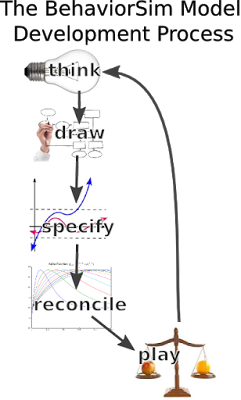
\includegraphics[width=0.5\columnwidth]{img/behaviorSim_process}  
  \caption{The five stages implemented in v1 of the behaviorSim Model Builder.}
  \label{model-builder-stages}
\end{figure}
  
The first iteration of the behaviorSim Model-Builder (see figure \ref{model-builder-v1}) took a step-wise approach to the task, which made backtracking difficult.

% [TODO picture of Model-Builder v0.1] 
\begin{figure}[!t]
  \centering
  1 
  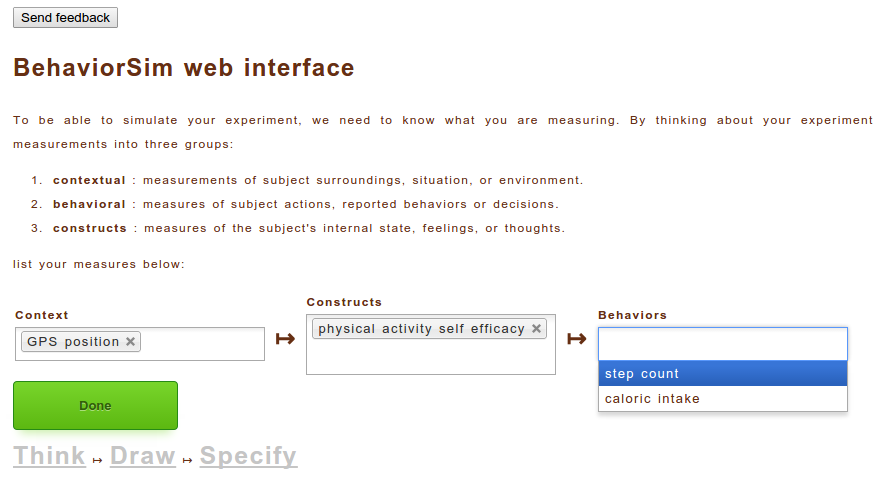
\includegraphics[width=0.9\columnwidth]{img/v1-think}
  \rule{\columnwidth}{0.4pt}
  2
  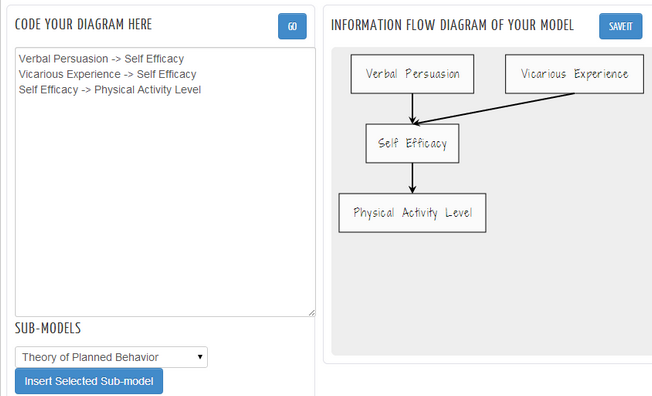
\includegraphics[width=0.9\columnwidth]{img/v1-draw}
  \rule{\columnwidth}{0.4pt}
  3
  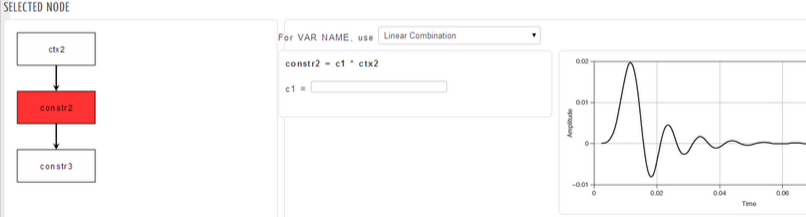
\includegraphics[width=0.9\columnwidth]{img/v1-specify}  
  \caption{behaviorSim Model Builder v0.1.x implemented three separate stages of model building as separate pages: 1) think, 2) draw, 3) specify.}
  \label{model-builder-v1}
\end{figure}

The model builder was tested using a think-aloud protocol with 2 behavioral scientists and 1 HCI expert. 
Though the steps in the outlined model development process are accurate, a step-wise design is not optimal.
Users who are forced to explore the process step-by-step have difficulty understanding how earlier choices related to later results, and feel constrained by previous choices rather than backtracking to revise the model.
This design does not allow for quick iteration on models, and requires the user to maintain a great deal of planning information internally.

Though the information flow diagram employed in this version worked well to convey information about the model to the users, the graph was also assumed to be interactive - participants made attempts to modify the graph by clicking, and attempted to select nodes in the specification stage by clicking on them.


\subsection{behaviorSim Model-Building Tutorial v1}
After reviewing v1 of the behaviorSim Model Builder too, a tutorial was designed to help bridge the knowledge gap for new modelers looking to use the tool.
In theory, the tutorial would help users see the bigger picture before diving into the step-wise process.

The tutorial was implemented as a walk-through of a simple model's internals.
The tutorial also introduced a hybridized information-flow and time-series graph, wherein each node of the graph contains a time-series spanning a common timeframe, and a user interface for adjusting model parameters and updating time-series values instantaneously.
 
\begin{figure}[!t]
  \centering
  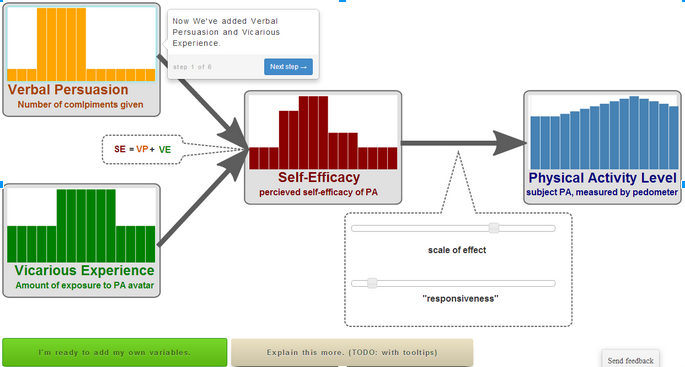
\includegraphics[width=0.9\columnwidth]{img/v1-flow}  
  \caption{behaviorSim Model Builder tutorial attempted to merge time-series and information-flow graph representations.}
  \label{model-builder-tutorial}
\end{figure}

The same think-aloud protocol as used for the evaluation of v1 of the model builder was used to evaluate this tutorial. 
Through this evaluation it became clear that even more explicit definition of terms was needed in order to clarify persistant diciplinary differences.

% TODO: See notes for more

\subsection{behaviorSim Model-Building Tool v2}
The second major version of the behaviorSim Model Building tool attempted to unify all steps of the modeling process (figure \ref{model-builder-stages}) into a single-page application.

\begin{figure}[!t]
  \centering
  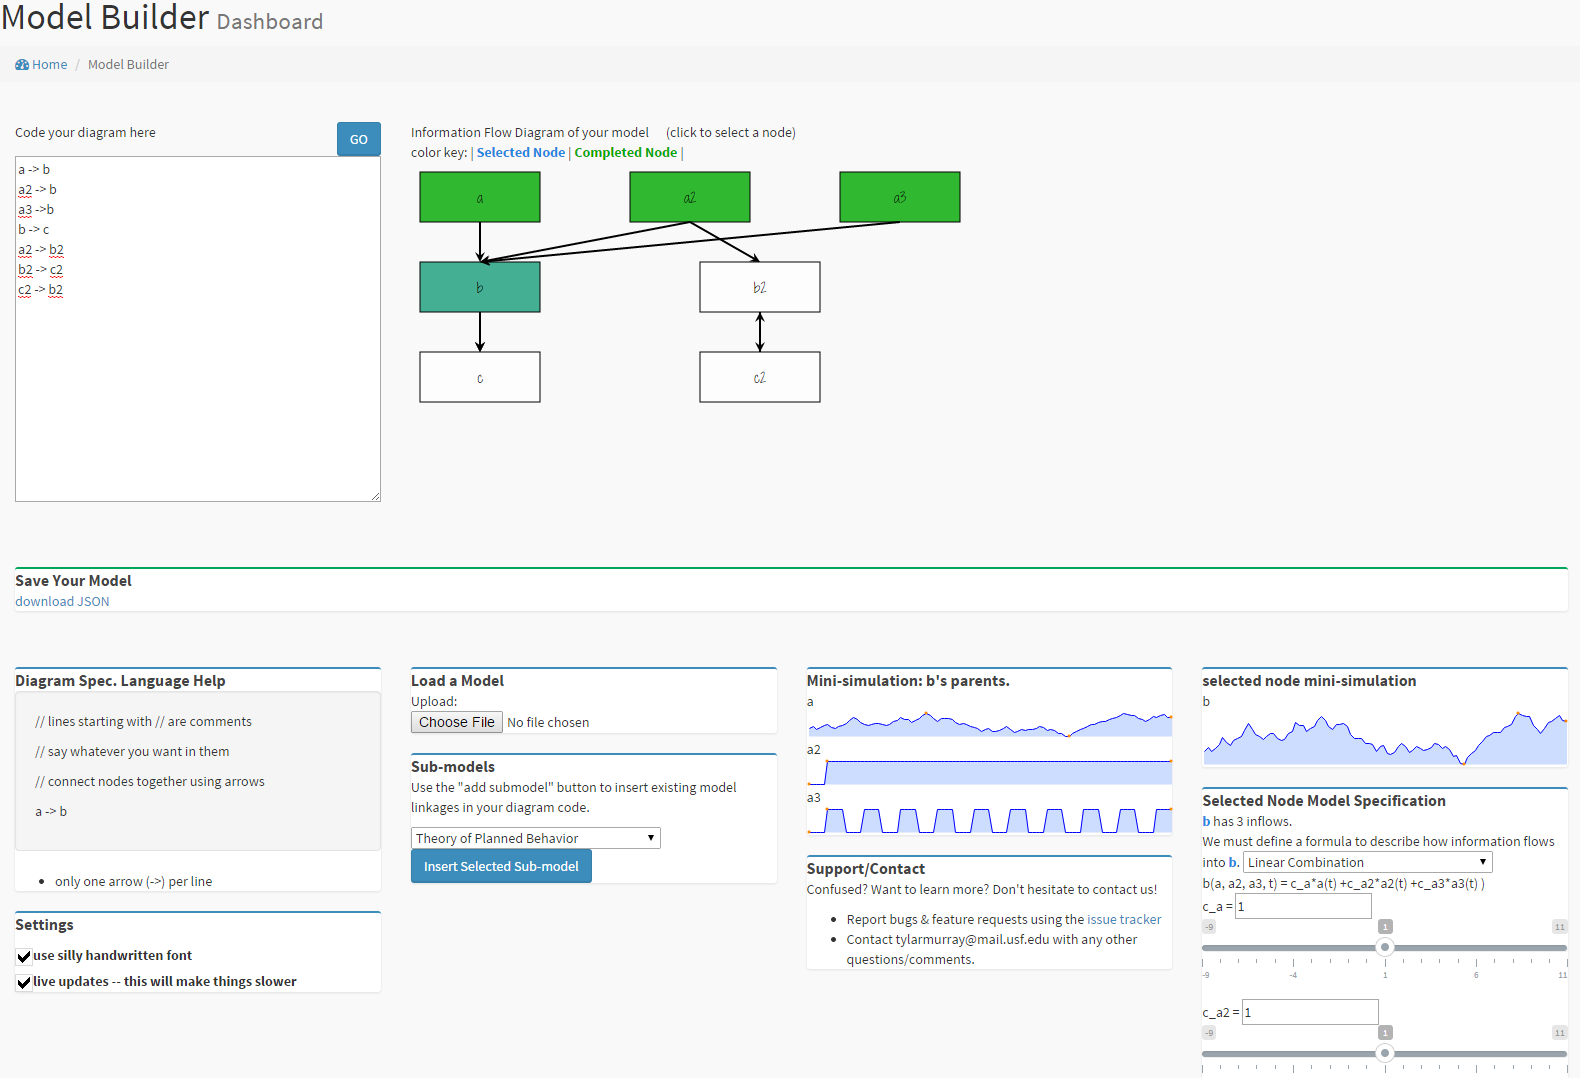
\includegraphics[width=0.9\columnwidth]{img/v2}  
  \caption{behaviorSim Model Builder v2 combines the think, draw, specify, and play elements into a single view.}
  \label{model-builder-v2}
\end{figure}

This version was again reviewed using a think-aloud protocol with 2 behavioral scientists, 1 HCI expert, and 1 behavioral modeler.

% TODO: see notes for more
  


  
\section{Design Guidelines}
Using lessons learned from our attempts at developing a model-building tool for behavioral modeling we propose a graph-based HBM specification, and provide generalized guidelines for developing modeling and simulation tools for behavioral scientists.

\subsection{HBM info-flow graph}
A "standard" approach to describing, designing, and visualizing human behavior models for personal forecasting is needed.
There are countless approaches to systems modeling, but concepts and methods ought to be incorporated and fused when possible in their application to behavioral science.
The resulting specification will allow for the formal description of a Human Behavior Model (HBM).

We will begin with the most basic definitions and then progress into the intricacies and usage examples of the proposed model-modeling paradigm.

A model is comprised of a network of variables and their interrelations.
In order to visually represent the connectivity of the model a network graph can be used.
Network graphs have many applications across multiple disciplines, and though the different implementations can be visually similar they can differ significantly in their meaning.
In general, however, a graph is comprised of nodes and edges which represent the variables and their connections, respectfully. 

We argue that the most intuitive representation is one which uses a directed graph wherein edge arrows to represent the flow of information between nodes.
Thus, a HBM  directed graph edge from node A to node B indicates that information flows from node A into node B. 

$A => B$

Graph 1: Can be read as "A influences B", "A informs B", or similar

This choice of notation is in agreement with graphs used in information theory, communications models, and behavioral science.
In contrast, some graphing paradigms (such as probabilistic graphical models) prefer to use notation wherein an edge is used to represent dependency.
In these paradigms edges may be read from tail to head as "depends on" or similar.

While the network graph does an excellent job showing the connectivity of a model, it fails to indicate the meaning of each connection.
In the majority of existing applications, the mathematical form of the relationship is implied or else it is neglected completely.
For instance, path diagrams from the behavioral sciences frequently denote dependence and do not specify functional form.
Adding even further to the confusion is the notion that these graphs are often developed using different statistical analyses which may make different assumptions about the functional definition of inter-variate dependency.
The most common analyses assess linear relationships between variables, and thus it is perhaps reasonable to assume that this is the intention of most authors.
Assuming this is the case we can return to our simplistic example in Graph 1 and interpret the implied relationship as:

$B = coeff_ab*A + const$

Equation 1: coeff represents the correlation coefficient which relates A to B, 
and const represents a scalar constant

For nodes with multiple inflow edges, such as node B in the following graph:

$A => B <= C => D$

Graph 2: Example; now with more nodes!

The resulting formulation is simply a sum of the inflows:

$B = coeff_ab*A + coeff_cb*C + const$

Equation 2: Combining multiple inflows via sum is referred to as the superposition principle and is the defining characteristic of linear systems (not to be confused with this linear formulation)

Using this formulation, the general form of our HBM is expressed via the network graph alone (perhaps along with a statement about what edges mean).
To express an ideographic implementation of this general model, we must also include a table of coefficient values. This representation is useful, but also very limited.
One important feature which this formulation does not take into account is the dynamics of the relationship.
This is very important for human behavior modeling because the variables in a HBM will often change their value over time.
Taking time into account our formulation for Graph 1 becomes:

$B(t) = coeff_ab*A(t) + const$

Looking at this closely we can note that at each point in time the value of A depends only on the value of B at that same instant in time.
This assumption is fine for many applications, but we argue that this is a very poor assumption for human behavior models. What if A is influenced by B but there is some lag before the effect manifests?
What if A is influenced by B, but only if B is above some threshold value? What if A is influenced by the rate of change in B rather than the value of B itself? All of these scenarios cannot be expressed using this simple linear relationship. 

To resolve some of these issues, a differential equations can be used to describe the relationship between variables as described by (CSEL paper which connects path diagrams and fluid-flow). Using the differential formulation our equation for Graph 1 becomes:

$B(t) = TODO..$

Just as before, our general model is not expressed entirely through the graph, and an ideographic example is specified by providing table of coefficient values.
Our table is now quite a bit larger, but these coefficients have meaningful definitions which relate to our theory.
While this formulation offers a huge improvement over the linear formulation, we can still imagine relationships which this formulation cannot express.
Thus, a graph-wide assumption that each edge represents a differential equation may not be general enough for our HBM specification. 

It should be noted at this point that although the linear formulation is too simple to express the dynamics of the differential formulation, the differential formulation is capable of expressing linear relationships.
This is accomplished by setting coefficients of dynamical components to 0.
One might think then that there is some general formula which could express any functional form and that this form should be used to express the relationships between variables in our HBM graphs.
While such formulations do exist (such as Taylor or Fourier series approximations or even ANN-based relations), this usage tends to make the model difficult to understand and to simulate with.
Indeed, linear and differential formulations are in such widespread use because of the relative ease with which we can understand and solve them. An additional problem raised by this approach is that of redundant formulations.
Indeed formulations could even subvert the "arrow direction" by drawing information contrary to our original choice of notation.
The graph can then no longer be considered a directed graph, and the meaning of an edge becomes less clear.
Additionally, the table of coefficients needed to express an ideographic case of the model quickly becomes prohibitively large, and the effect of each coefficient on the outcome is not intuitively meaningful.

Let us now consider the case where a graph-wide assumption is NOT made.
That is, we will specify the functional form of each node individually so that each edge on the graph may be linear in form while another may be differential.
This has the benefit of allowing for both complex relationships between variables as well as simplistic ones.
In this way one could craft a model in which two variables are linearly related and a third is dependent on the variance of another variable (a particularly odd formulation, but one which is relevant to behavioral theory).
Unfortunately, this approach also means that a table of formulations must now be included with our graph to show the meaning of each edge in the graph.
Consider for example the table below for Graph 2:

\begin{centering}
\begin{tabular}{ | l | l | l |}
    \hline
    node & formulation \\ \hline
    B & $coeff_ab*A(t) + coeff_cb*C(t) + cosnst$  \\ \hline
    D & $ TODO $ \\ \hline
\end{tabular}
Table 1: an example formulation table for Graph 2 
\end{centering}


If a fixed number of functional forms is adhered to, the graph can be made to visually represent these functional forms through the use of different node icon shapes. 
This approach quickly begins to resemble applications which use flow-based programming. 
Indeed, they are quite similar in their approach, and the specification of a HBM is quite similar to the writing of a program.

Note also that a node can set any arbitrary formulation if needed. 
This is the least desirable situation, since the meaning of an inflow to each node even more convoluted. 
Though this usage reduces the ability of the graph to reduce processing load on the user through abstraction, there may be some cases where this type of formulation is desirable. 
Consider the following graph and formulation table:

$A => B <= C => D => E$

Graph 3: The final example graph.

\begin{centering}
\begin{tabular}{ | l | l | l |}
    \hline
    node & formulation \\ \hline
    B & $coeff_ab*A(t) + coeff_cb*sqrt(C(t)) + const_b$ \\ \hline
    D & $ TODO $ \\ \hline
    E & $coeff_de*D(t) + const_de$ \\ \hline
\end{tabular}
Table 2: an example formulation table for Graph 3
\end{centering}

In conclusion, we propose that an HBM should be specified using the following rules:
% TODO: convert these to item-lists

\begin{enumerate}
  \item use a graph-wide formula assumption if possible
  \item when choosing a formulation, consistency between nodes is most important
  \item when choosing a formulation, simplicity and clarity is second only to consistency
  \item Thus a HBM specification must include:
  \begin{enumerate}
   \item An information flow graph
   \item one of:
    \begin{itemize}
      \item a graph-wide formulaic assumption
      \item a formulation table 
    \end{itemize}
  \end{enumerate}
\end{enumerate}

In order to express a particular solution of a general HBM, an ideographic HBM must also include a table of coefficient values. 

\subsection{Tool Design Guidelines}
The guidelines provided below are generalizable findings from our studies which may be useful for other developing modeling and simulation tools for behavioral scientists.


Ease of use and intuitive user interface is a primary design consideration for existing softwares for modeling and simulation in systems theory. (reference and cite vensim, etc, from here) 
The ease of use of a system is one of the most important factors in the adoption of the system. (cite technology acceptance model?) 
The trans-disciplinary nature of a human-behavior modeling toolkit may require special consideration in order to be usable by those who may be unfamiliar with modeling and simulation concepts.

TODO: Figure: path2flow.png example of the rise in model complexity for the theory of planned behavior when mathematical assumptions are made explicit. (from: Ajzen 1985,1991,2002 (left), Nandola et al. 2013 (right))

(overview and definitions)

* information-searching / focus and context design

* walk-through first use instead of tutorial (see, copy, do) /cite{?}

* use existing terminology (but also define it)

* a summary of lessons learned and suggestions for future works

* multipage vs single-page (v0.1->v0.2)

* inquiries in panel-reviews

* single-page is overwhelming 

* multiple terminologies from user surveys /cite{ontology} customizable? 





\section{Proposed Tool: Model-Builder v3}
* noflo, flow-based programming style
* how does this new design use the design guidelines outlined?

\begin{figure}[!t]
  \centering
  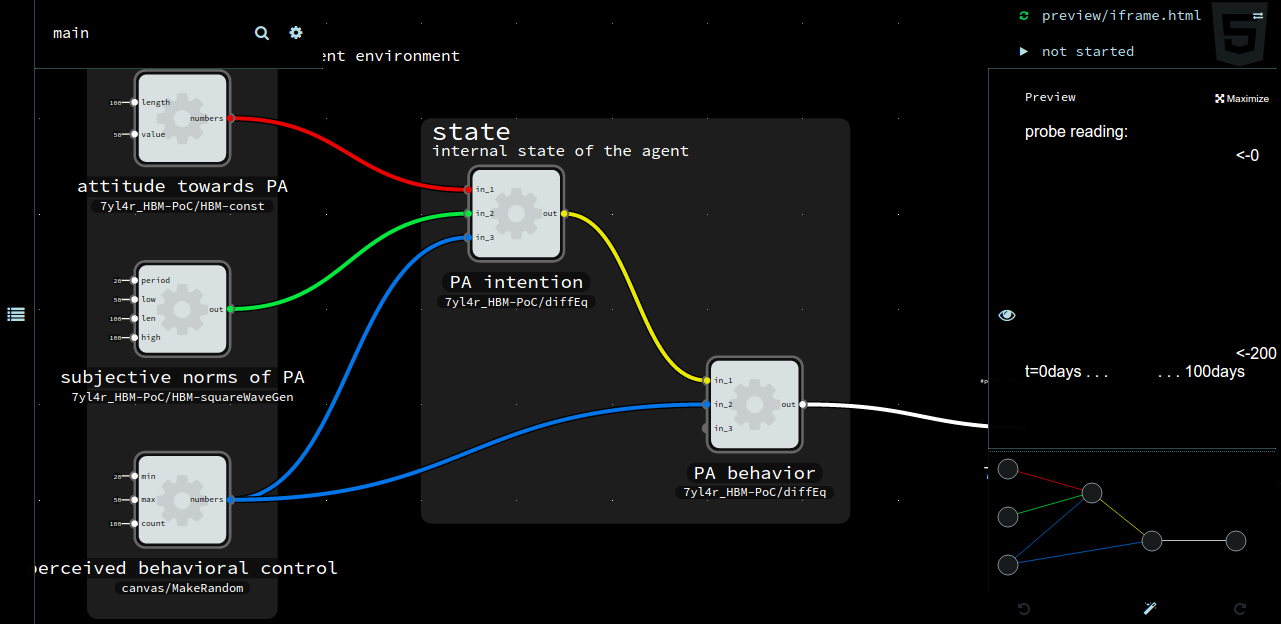
\includegraphics[width=0.9\columnwidth]{img/v3}  
  \caption{behaviorSim Model Builder v3 brings increased focus onto the graph using a flow-based programming approach.}
  \label{model-builder-v3}
\end{figure}


\subsection{User Interface Design for HBM-builder }
The flow chart shown in figure \ref{HBM-build-process} represents the movement of a user through the process of building an HBM, or any graphical model for that matter.

\begin{figure}[!t]
  \centering
  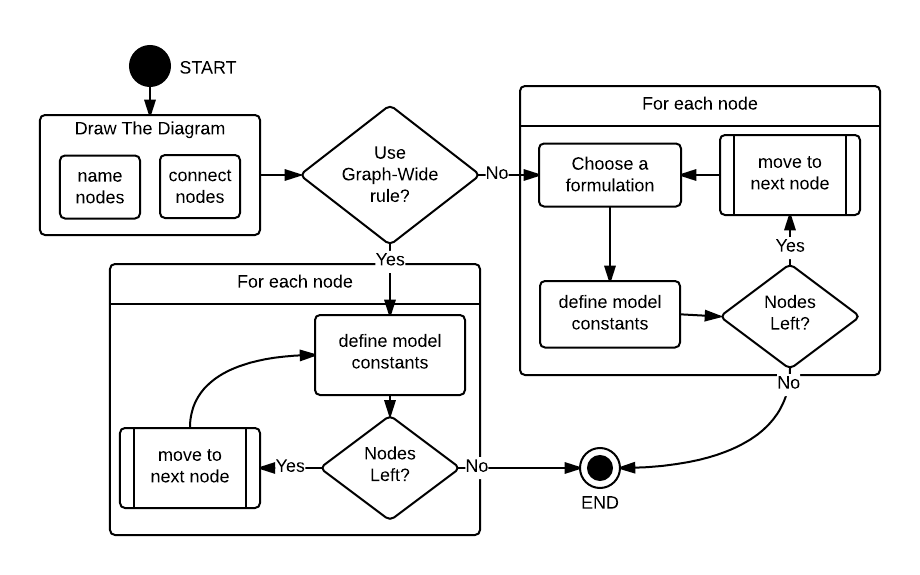
\includegraphics[width=0.9\columnwidth]{img/HBM-build-process}
  \caption{Flow chart depicting the process of building a graphical HBM.}
  \label{HBM-build-process}
\end{figure}

It is important to note that the process of building is pseudo-linear; users will likely want to jump back to an arbitrary point in the process and as the model takes shape. 
As the user moves through the process, they will re-assess the meaning of variables and connections and their model will solidify. 
UI for an HBM-building tool should enable easy backtracking and should work to provide feedback on the characteristics of the model early. 

%TODO: move this:
The second generation of the Model Builder Tool presents a guided process which takes place within a single-page application. 
In this way, users can see how choices influence the model in real-time, and thus can iterate on their design much sooner.

While keeping the non-linearity of this process in mind, we will now walk through the diagram and address design considerations for each part of the process.

\subsubsection{Draw the Diagram}
This task involves the creation and connecting of all nodes in the diagram. 
Nodes and their connections should be primarily based in theory, so a user should be able to build a first draft of their model with little feedback. 
Once the formulas for each node have been specified, however, it is likely that the user will want to return to this step and reassess the network. 
Several paradigms diagram-drawing have been well tested, but there are essentially two prevailing options:
1) drag-and-drop node creation with drag-to-connect edges, and 2) textual ``diagram specification language''.

\paragraph{drag-and-connect}
pros:
\begin{enumerate}
  \item{easy and intuitive to use}
\end{enumerate}
cons:
\begin{enumerate}
 \item can be difficult to position nodes to reduce edge overlap
 \item users often distracted trying to make graph "pretty"
 \item requires constant switching between mouse and keyboard2
\end{enumerate}

\paragraph{Diagram Specification Language}
pros:
\begin{enumerate}
 \item can be much faster than mouse-based
 \item searching/finding nodes for modification is as easy as textual search
\end{enumerate}

cons:
\begin{enumerate}
 \item parsing errors can be a source of confusion
 \item user must learn the markup "language"
\end{enumerate}

\subsubsection{Use Graph-Wide Rule?}
This choice can come before or after the initial drawing of the graph, since it is likely the user has a graph-wide assumption in mind when starting the process. 
This choice determines whether or not the interface for specifying nodes individually is shown, so it is logical to think of the "none", "node-specific", or "node-unique" option as one of the choices available here. 

As an example, some graph-wide rules which may be implemented include:
\begin{enumerate}
  \item Probabilistic Graphical Network
  \item Linear Sum
  \item Fluid-Flow Analogy / Differential Equation Formulation (1st order and 2nd order)
\end{enumerate}

If a graph-wide rule is set, the formulation section for each node should show as locked to the rule's respective formulation. 
Editing an individual node's formulation will disable the graph-wide rule, and should require confirmation from the user. 

The interface for choosing one of these rules may be as simple as a select-option box or may include a detailed rule description and example. 

An additional feature which may be useful is to allow for user-defined graph-wide rules. 
In this case, users might choose "create new rule" and an interface to allow users to edit and save graph-wide rules is needed.

\subsubsection{For Each Node}

Items encapsulated by the "for each node" swim-lanes must be executed for each node in the graph. 
The graph-wide-rule-yes case differs from the graph-wide-rule-no case only in that the graph-wide-rule-no case requires the additional step of setting the formulation at each node.

\subsubsection{Choose a Formulation}
This item is identical to the graph-wide rule choice, except that it applies only to a single node. Similar design considerations apply, and user-defined choice is even more important at this scale.

\subsubsection{Define Model Constants}
The general solution of an HBM does not require definition of the constants, but a simulation cannot be run until some numerical value is assumed. 
These constants often have theoretical significance in that they often have meaningful influence upon system behavior. 
Scaling-coefficients, for instance allow for relative weighting of each inflow. 
Similarly, the coefficients of a dynamical equation define how quickly variables react to a change "upstream". 

UI for setting these constants could be as simple as a numerical input for each coefficient's name, but additional model details provided here may be of great benefit to the model designer. 

Firstly, UI should include equation-specific descriptions of the constants whenever possible. This means that a separate UI for each formulation type is necessary. 

Secondly, adjustment of coefficients would ideally show changes in the dynamics of a node's value in real-time. 
This can take the form of a time-series chart of the selected node's numerical value over time along with (editable) time-series for the inflows. 
Adjustment of these inflow series may also take a number of different forms. 

Thirdly, model creators may want to set these coefficients in three different ways: 
\paragraph{1) Set the coefficient value to a constant}
All simulations derived from this general solution will have this exact value.

\paragraph{2) Set a probability distribution for the coefficient}
Simulations derived from this general solution will select a numerical value based on the given distribution. 
This distribution may be learned from a training dataset, or bounds may be set for later training. 

\paragraph{3) Leave the variable unbounded and assume a flat probability distribution}
This selection is identical to option 2 with a flat distribution from -infinity to +infinity.


These different ways of defining coefficients in a HBM become very important when it is time to run simulations and compare model results to real data. 

Lastly, model creators may want to use a measured value to set the value of these coefficients. In this way, one measured input (in real life), such as big-5 personality type, can be used to set the value of multiple coefficients across different variables in the model.

% Designing UI for the model-constant-defining process is complex enough to warrant it's own article, which I will write later and link to here(TODO).

\subsubsection{Nodes Left?}
%This is the most simple element of the flowchart. 
No if there are un-specified nodes remaining, yes if all are complete. 
It should be left to the user to confirm model-completeness, however, since a great deal of model-tweaking is likely now that simulation results can be displayed.

\subsubsection{Next Node}
Progression downstream through the model should be relatively straightforward in the case of tree-like models, but feedback loops can cause issues here. 
Perhaps the best paradigm here is to progress as naturally as possible, but allow the user to over-ride and select any node. 
This interaction mode is needed to allow for later model-tweaking anyway. 

The behaviorSim Model Builder v0.2 currently does not include significant enough indicator of node "completeness", so that the user is sometimes unsure when they should feel free to move to the next node.




\section{Conclusion}
We have provided design guidelines to aid in development of modeling and simulation tools for behavioral scientists based on lessons learned in the development process, and have outlined the design of an application which utilizes these guidelines.



% An example of a floating figure using the graphicx package.
% Note that \label must occur AFTER (or within) \caption.
% For figures, \caption should occur after the \includegraphics.
% Note that IEEEtran v1.7 and later has special internal code that
% is designed to preserve the operation of \label within \caption
% even when the captionsoff option is in effect. However, because
% of issues like this, it may be the safest practice to put all your
% \label just after \caption rather than within \caption{}.
%
% Reminder: the "draftcls" or "draftclsnofoot", not "draft", class
% option should be used if it is desired that the figures are to be
% displayed while in draft mode.
%
%\begin{figure}[!t]
%\centering
%\includegraphics[width=2.5in]{myfigure}
% where an .eps filename suffix will be assumed under latex, 
% and a .pdf suffix will be assumed for pdflatex; or what has been declared
% via \DeclareGraphicsExtensions.
%\caption{Simulation Results}
%\label{fig_sim}
%\end{figure}

% Note that IEEE typically puts floats only at the top, even when this
% results in a large percentage of a column being occupied by floats.


% An example of a double column floating figure using two subfigures.
% (The subfig.sty package must be loaded for this to work.)
% The subfigure \label commands are set within each subfloat command, the
% \label for the overall figure must come after \caption.
% \hfil must be used as a separator to get equal spacing.
% The subfigure.sty package works much the same way, except \subfigure is
% used instead of \subfloat.
%
%\begin{figure*}[!t]
%\centerline{\subfloat[Case I]\includegraphics[width=2.5in]{subfigcase1}%
%\label{fig_first_case}}
%\hfil
%\subfloat[Case II]{\includegraphics[width=2.5in]{subfigcase2}%
%\label{fig_second_case}}}
%\caption{Simulation results}
%\label{fig_sim}
%\end{figure*}
%
% Note that often IEEE papers with subfigures do not employ subfigure
% captions (using the optional argument to \subfloat), but instead will
% reference/describe all of them (a), (b), etc., within the main caption.


% An example of a floating table. Note that, for IEEE style tables, the 
% \caption command should come BEFORE the table. Table text will default to
% \footnotesize as IEEE normally uses this smaller font for tables.
% The \label must come after \caption as always.
%
%\begin{table}[!t]
%% increase table row spacing, adjust to taste
%\renewcommand{\arraystretch}{1.3}
% if using array.sty, it might be a good idea to tweak the value of
% \extrarowheight as needed to properly center the text within the cells
%\caption{An Example of a Table}
%\label{table_example}
%\centering
%% Some packages, such as MDW tools, offer better commands for making tables
%% than the plain LaTeX2e tabular which is used here.
%\begin{tabular}{|c||c|}
%\hline
%One & Two\\
%\hline
%Three & Four\\
%\hline
%\end{tabular}
%\end{table}


% Note that IEEE does not put floats in the very first column - or typically
% anywhere on the first page for that matter. Also, in-text middle ("here")
% positioning is not used. Most IEEE journals/conferences use top floats
% exclusively. Note that, LaTeX2e, unlike IEEE journals/conferences, places
% footnotes above bottom floats. This can be corrected via the \fnbelowfloat
% command of the stfloats package.


% conference papers do not normally have an appendix


% use section* for acknowledgement
%\section*{Acknowledgment}
%The authors would like to thank...


% trigger a \newpage just before the given reference
% number - used to balance the columns on the last page
% adjust value as needed - may need to be readjusted if
% the document is modified later
%\IEEEtriggeratref{8}
% The "triggered" command can be changed if desired:
%\IEEEtriggercmd{\enlargethispage{-5in}}

% references section

% can use a bibliography generated by BibTeX as a .bbl file
% BibTeX documentation can be easily obtained at:
% http://www.ctan.org/tex-archive/biblio/bibtex/contrib/doc/
% The IEEEtran BibTeX style support page is at:
% http://www.michaelshell.org/tex/ieeetran/bibtex/
\bibliographystyle{IEEEtran}
% argument is your BibTeX string definitions and bibliography database(s)
\bibliography{IEEEabrv,main}
%
% <OR> manually copy in the resultant .bbl file
% set second argument of \begin to the number of references
% (used to reserve space for the reference number labels box)
% \begin{thebibliography}{1}
% 
% \bibitem{IEEEhowto:kopka}
% H.~Kopka and P.~W. Daly, \emph{A Guide to \LaTeX}, 3rd~ed.\hskip 1em plus
%   0.5em minus 0.4em\relax Harlow, England: Addison-Wesley, 1999.
% 
% \end{thebibliography}




% that's all folks
\end{document}


